\documentclass[1p]{elsarticle_modified}
%\bibliographystyle{elsarticle-num}

%\usepackage[colorlinks]{hyperref}
%\usepackage{abbrmath_seonhwa} %\Abb, \Ascr, \Acal ,\Abf, \Afrak
\usepackage{amsfonts}
\usepackage{amssymb}
\usepackage{amsmath}
\usepackage{amsthm}
\usepackage{scalefnt}
\usepackage{amsbsy}
\usepackage{kotex}
\usepackage{caption}
\usepackage{subfig}
\usepackage{color}
\usepackage{graphicx}
\usepackage{xcolor} %% white, black, red, green, blue, cyan, magenta, yellow
\usepackage{float}
\usepackage{setspace}
\usepackage{hyperref}

\usepackage{tikz}
\usetikzlibrary{arrows}

\usepackage{multirow}
\usepackage{array} % fixed length table
\usepackage{hhline}

%%%%%%%%%%%%%%%%%%%%%
\makeatletter
\renewcommand*\env@matrix[1][\arraystretch]{%
	\edef\arraystretch{#1}%
	\hskip -\arraycolsep
	\let\@ifnextchar\new@ifnextchar
	\array{*\c@MaxMatrixCols c}}
\makeatother %https://tex.stackexchange.com/questions/14071/how-can-i-increase-the-line-spacing-in-a-matrix
%%%%%%%%%%%%%%%

\usepackage[normalem]{ulem}

\newcommand{\msout}[1]{\ifmmode\text{\sout{\ensuremath{#1}}}\else\sout{#1}\fi}
%SOURCE: \msout is \stkout macro in https://tex.stackexchange.com/questions/20609/strikeout-in-math-mode

\newcommand{\cancel}[1]{
	\ifmmode
	{\color{red}\msout{#1}}
	\else
	{\color{red}\sout{#1}}
	\fi
}

\newcommand{\add}[1]{
	{\color{blue}\uwave{#1}}
}

\newcommand{\replace}[2]{
	\ifmmode
	{\color{red}\msout{#1}}{\color{blue}\uwave{#2}}
	\else
	{\color{red}\sout{#1}}{\color{blue}\uwave{#2}}
	\fi
}

\newcommand{\Sol}{\mathcal{S}} %segment
\newcommand{\D}{D} %diagram
\newcommand{\A}{\mathcal{A}} %arc


%%%%%%%%%%%%%%%%%%%%%%%%%%%%%5 test

\def\sl{\operatorname{\textup{SL}}(2,\Cbb)}
\def\psl{\operatorname{\textup{PSL}}(2,\Cbb)}
\def\quan{\mkern 1mu \triangleright \mkern 1mu}

\theoremstyle{definition}
\newtheorem{thm}{Theorem}[section]
\newtheorem{prop}[thm]{Proposition}
\newtheorem{lem}[thm]{Lemma}
\newtheorem{ques}[thm]{Question}
\newtheorem{cor}[thm]{Corollary}
\newtheorem{defn}[thm]{Definition}
\newtheorem{exam}[thm]{Example}
\newtheorem{rmk}[thm]{Remark}
\newtheorem{alg}[thm]{Algorithm}

\newcommand{\I}{\sqrt{-1}}
\begin{document}

%\begin{frontmatter}
%
%\title{Boundary parabolic representations of knots up to 8 crossings}
%
%%% Group authors per affiliation:
%\author{Yunhi Cho} 
%\address{Department of Mathematics, University of Seoul, Seoul, Korea}
%\ead{yhcho@uos.ac.kr}
%
%
%\author{Seonhwa Kim} %\fnref{s_kim}}
%\address{Center for Geometry and Physics, Institute for Basic Science, Pohang, 37673, Korea}
%\ead{ryeona17@ibs.re.kr}
%
%\author{Hyuk Kim}
%\address{Department of Mathematical Sciences, Seoul National University, Seoul 08826, Korea}
%\ead{hyukkim@snu.ac.kr}
%
%\author{Seokbeom Yoon}
%\address{Department of Mathematical Sciences, Seoul National University, Seoul, 08826,  Korea}
%\ead{sbyoon15@snu.ac.kr}
%
%\begin{abstract}
%We find all boundary parabolic representation of knots up to 8 crossings.
%
%\end{abstract}
%\begin{keyword}
%    \MSC[2010] 57M25 
%\end{keyword}
%
%\end{frontmatter}

%\linenumbers
%\tableofcontents
%
\newcommand\colored[1]{\textcolor{white}{\rule[-0.35ex]{0.8em}{1.4ex}}\kern-0.8em\color{red} #1}%
%\newcommand\colored[1]{\textcolor{white}{ #1}\kern-2.17ex	\textcolor{white}{ #1}\kern-1.81ex	\textcolor{white}{ #1}\kern-2.15ex\color{red}#1	}

{\Large $\underline{12a_{0414}~(K12a_{0414})}$}

\setlength{\tabcolsep}{10pt}
\renewcommand{\arraystretch}{1.6}
\vspace{1cm}\begin{tabular}{m{100pt}>{\centering\arraybackslash}m{274pt}}
\multirow{5}{120pt}{
	\centering
	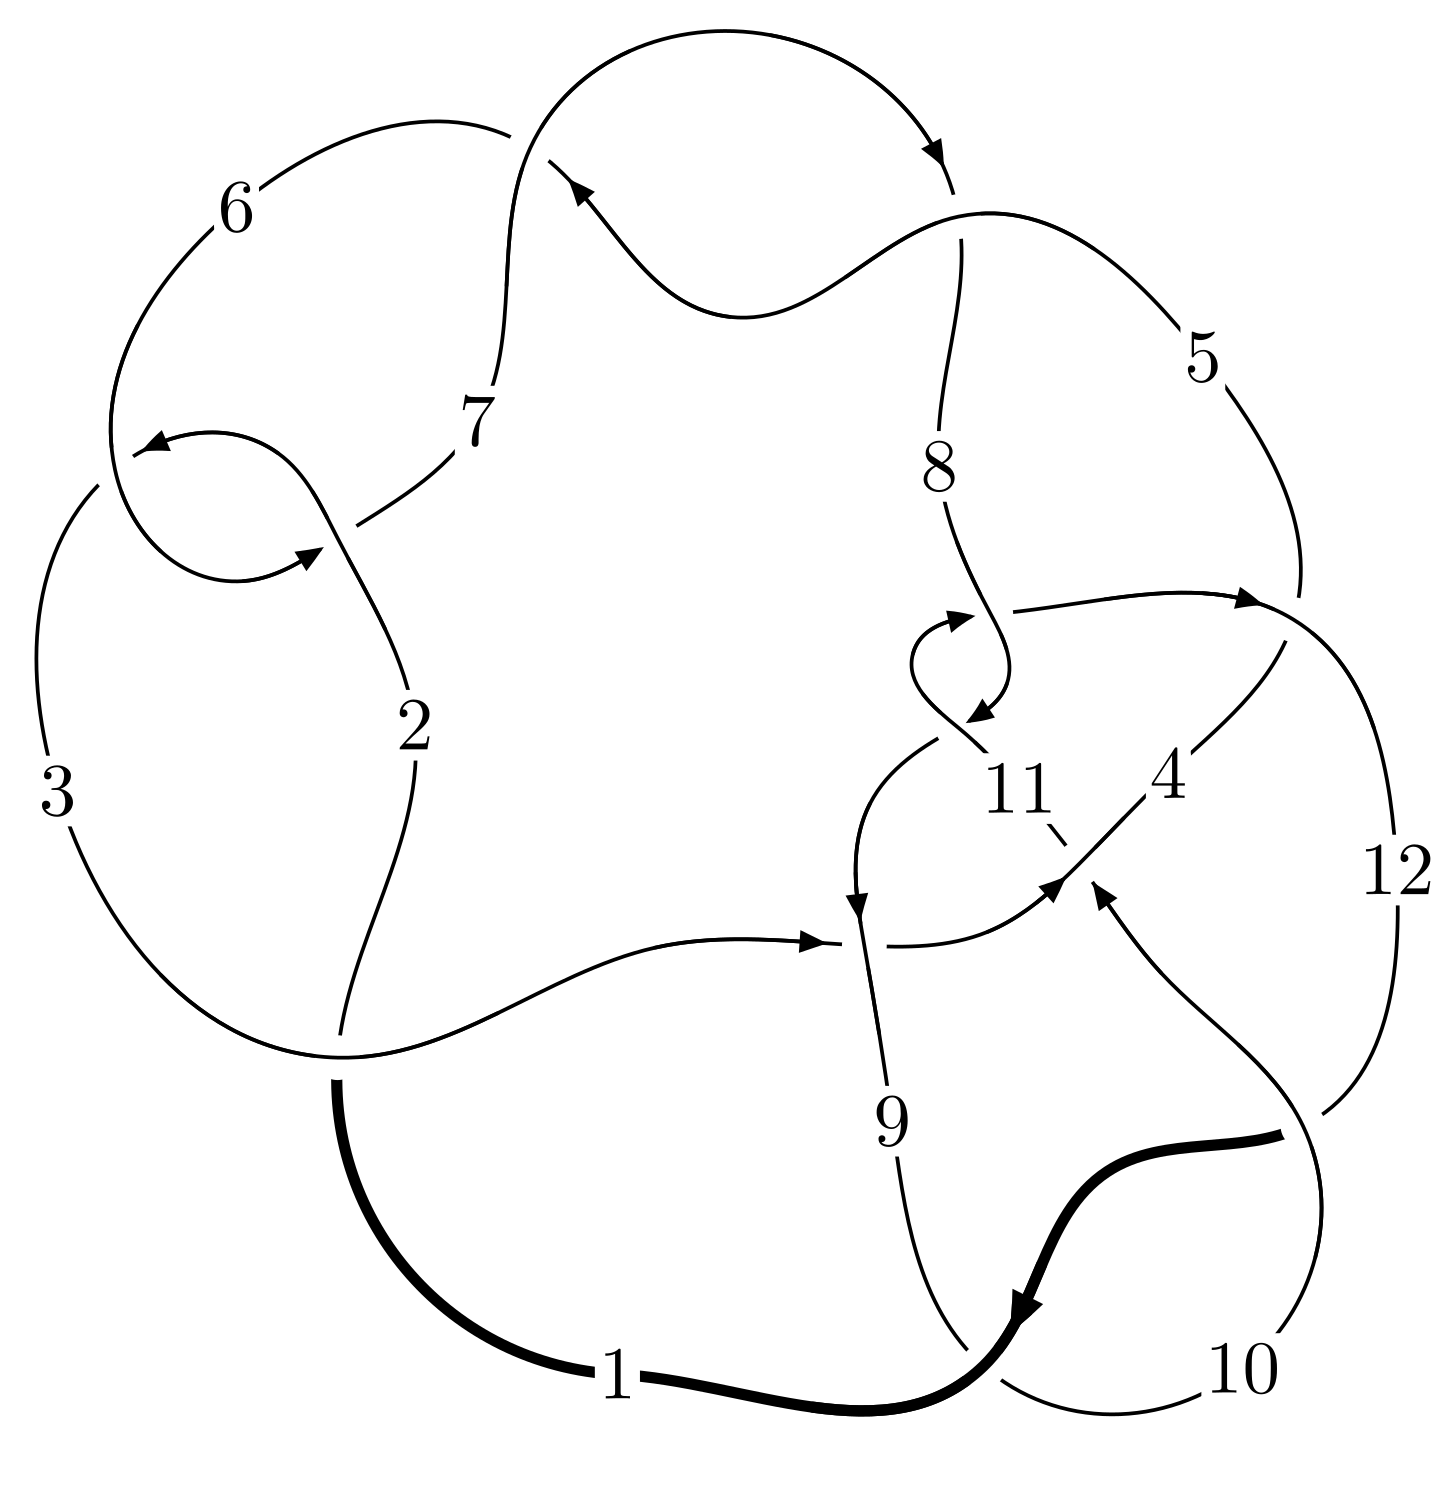
\includegraphics[width=112pt]{../../../GIT/diagram.site/Diagrams/png/1215_12a_0414.png}\\
\ \ \ A knot diagram\footnotemark}&
\allowdisplaybreaks
\textbf{Linearized knot diagam} \\
\cline{2-2}
 &
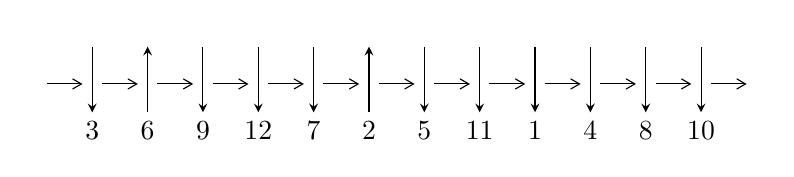
\begin{tikzpicture}[x=20pt, y=17pt]
	% nodes
	\node (C0) at (0, 0) {};
	\node (C1) at (1, 0) {};
	\node (C1U) at (1, +1) {};
	\node (C1D) at (1, -1) {3};

	\node (C2) at (2, 0) {};
	\node (C2U) at (2, +1) {};
	\node (C2D) at (2, -1) {6};

	\node (C3) at (3, 0) {};
	\node (C3U) at (3, +1) {};
	\node (C3D) at (3, -1) {9};

	\node (C4) at (4, 0) {};
	\node (C4U) at (4, +1) {};
	\node (C4D) at (4, -1) {12};

	\node (C5) at (5, 0) {};
	\node (C5U) at (5, +1) {};
	\node (C5D) at (5, -1) {7};

	\node (C6) at (6, 0) {};
	\node (C6U) at (6, +1) {};
	\node (C6D) at (6, -1) {2};

	\node (C7) at (7, 0) {};
	\node (C7U) at (7, +1) {};
	\node (C7D) at (7, -1) {5};

	\node (C8) at (8, 0) {};
	\node (C8U) at (8, +1) {};
	\node (C8D) at (8, -1) {11};

	\node (C9) at (9, 0) {};
	\node (C9U) at (9, +1) {};
	\node (C9D) at (9, -1) {1};

	\node (C10) at (10, 0) {};
	\node (C10U) at (10, +1) {};
	\node (C10D) at (10, -1) {4};

	\node (C11) at (11, 0) {};
	\node (C11U) at (11, +1) {};
	\node (C11D) at (11, -1) {8};

	\node (C12) at (12, 0) {};
	\node (C12U) at (12, +1) {};
	\node (C12D) at (12, -1) {10};
	\node (C13) at (13, 0) {};

	% arrows
	\draw[->,>={angle 60}]
	(C0) edge (C1) (C1) edge (C2) (C2) edge (C3) (C3) edge (C4) (C4) edge (C5) (C5) edge (C6) (C6) edge (C7) (C7) edge (C8) (C8) edge (C9) (C9) edge (C10) (C10) edge (C11) (C11) edge (C12) (C12) edge (C13) ;	\draw[->,>=stealth]
	(C1U) edge (C1D) (C2D) edge (C2U) (C3U) edge (C3D) (C4U) edge (C4D) (C5U) edge (C5D) (C6D) edge (C6U) (C7U) edge (C7D) (C8U) edge (C8D) (C9U) edge (C9D) (C10U) edge (C10D) (C11U) edge (C11D) (C12U) edge (C12D) ;
	\end{tikzpicture} \\
\hhline{~~} \\& 
\textbf{Solving Sequence} \\ \cline{2-2} 
 &
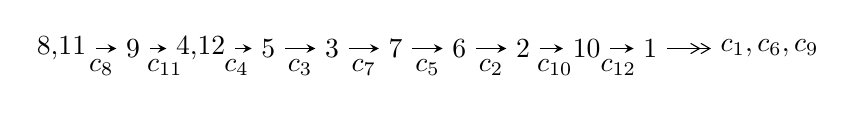
\begin{tikzpicture}[x=23pt, y=7pt]
	% node
	\node (A0) at (-1/8, 0) {8,11};
	\node (A1) at (1, 0) {9};
	\node (A2) at (33/16, 0) {4,12};
	\node (A3) at (25/8, 0) {5};
	\node (A4) at (33/8, 0) {3};
	\node (A5) at (41/8, 0) {7};
	\node (A6) at (49/8, 0) {6};
	\node (A7) at (57/8, 0) {2};
	\node (A8) at (65/8, 0) {10};
	\node (A9) at (73/8, 0) {1};
	\node (C1) at (1/2, -1) {$c_{8}$};
	\node (C2) at (3/2, -1) {$c_{11}$};
	\node (C3) at (21/8, -1) {$c_{4}$};
	\node (C4) at (29/8, -1) {$c_{3}$};
	\node (C5) at (37/8, -1) {$c_{7}$};
	\node (C6) at (45/8, -1) {$c_{5}$};
	\node (C7) at (53/8, -1) {$c_{2}$};
	\node (C8) at (61/8, -1) {$c_{10}$};
	\node (C9) at (69/8, -1) {$c_{12}$};
	\node (A10) at (11, 0) {$c_{1},c_{6},c_{9}$};

	% edge
	\draw[->,>=stealth]	
	(A0) edge (A1) (A1) edge (A2) (A2) edge (A3) (A3) edge (A4) (A4) edge (A5) (A5) edge (A6) (A6) edge (A7) (A7) edge (A8) (A8) edge (A9) ;
	\draw[->>,>={angle 60}]	
	(A9) edge (A10);
\end{tikzpicture} \\ 

\end{tabular} \\

\footnotetext{
The image of knot diagram is generated by the software ``\textbf{Draw programme}" developed by Andrew Bartholomew(\url{http://www.layer8.co.uk/maths/draw/index.htm\#Running-draw}), where we modified some parts for our purpose(\url{https://github.com/CATsTAILs/LinksPainter}).
}\phantom \\ \newline 
\centering \textbf{Ideals for irreducible components\footnotemark of $X_{\text{par}}$} 
 
\begin{align*}
I^u_{1}&=\langle 
5989 u^{32}-10457 u^{31}+\cdots+131072 b-109701,\;4909 u^{32}-21209 u^{31}+\cdots+8192 a-2485,\\
\phantom{I^u_{1}}&\phantom{= \langle  }u^{33}-4 u^{32}+\cdots-5 u-1\rangle \\
I^u_{2}&=\langle 
-1.96974\times10^{53} u^{47}-1.99921\times10^{54} u^{46}+\cdots+5.08812\times10^{53} b-4.24069\times10^{53},\\
\phantom{I^u_{2}}&\phantom{= \langle  }-5.78567\times10^{53} u^{47}-4.93093\times10^{54} u^{46}+\cdots+5.08812\times10^{53} a-2.96282\times10^{54},\\
\phantom{I^u_{2}}&\phantom{= \langle  }u^{48}+9 u^{47}+\cdots+64 u^2+1\rangle \\
I^u_{3}&=\langle 
16 b^4+8 b^3+12 b^2+4 b+1,\;a,\;u-1\rangle \\
I^u_{4}&=\langle 
a u+b- u+1,\;a^2- a+1,\;u^2+1\rangle \\
\\
\end{align*}
\raggedright * 4 irreducible components of $\dim_{\mathbb{C}}=0$, with total 89 representations.\\
\footnotetext{All coefficients of polynomials are rational numbers. But the coefficients are sometimes approximated in decimal forms when there is not enough margin.}
\newpage
\renewcommand{\arraystretch}{1}
\centering \section*{I. $I^u_{1}= \langle 5989 u^{32}-10457 u^{31}+\cdots+131072 b-109701,\;4909 u^{32}-21209 u^{31}+\cdots+8192 a-2485,\;u^{33}-4 u^{32}+\cdots-5 u-1 \rangle$}
\flushleft \textbf{(i) Arc colorings}\\
\begin{tabular}{m{7pt} m{180pt} m{7pt} m{180pt} }
\flushright $a_{8}=$&$\begin{pmatrix}1\\0\end{pmatrix}$ \\
\flushright $a_{11}=$&$\begin{pmatrix}0\\u\end{pmatrix}$ \\
\flushright $a_{9}=$&$\begin{pmatrix}1\\u^2\end{pmatrix}$ \\
\flushright $a_{4}=$&$\begin{pmatrix}-0.599243 u^{32}+2.58899 u^{31}+\cdots+10.0874 u+0.303345\\-0.0456924 u^{32}+0.0797806 u^{31}+\cdots+2.44522 u+0.836952\end{pmatrix}$ \\
\flushright $a_{12}=$&$\begin{pmatrix}- u\\u\end{pmatrix}$ \\
\flushright $a_{5}=$&$\begin{pmatrix}-0.470421 u^{32}+1.90313 u^{31}+\cdots+10.2872 u+0.214317\\-0.174515 u^{32}+0.765640 u^{31}+\cdots+2.24542 u+0.925980\end{pmatrix}$ \\
\flushright $a_{3}=$&$\begin{pmatrix}-0.688271 u^{32}+3.07392 u^{31}+\cdots+12.1718 u+0.948280\\-0.216263 u^{32}+0.632584 u^{31}+\cdots+3.00031 u+0.965775\end{pmatrix}$ \\
\flushright $a_{7}=$&$\begin{pmatrix}-0.0625076 u^{32}+0.312538 u^{31}+\cdots-3.24997 u+1.93751\\0.0625153 u^{32}-0.312576 u^{31}+\cdots-0.750061 u+0.0624847\end{pmatrix}$ \\
\flushright $a_{6}=$&$\begin{pmatrix}0.183983 u^{32}-0.905144 u^{31}+\cdots+6.21585 u-1.95071\\0.0234833 u^{32}-0.0922699 u^{31}+\cdots+0.322815 u-0.177536\end{pmatrix}$ \\
\flushright $a_{2}=$&$\begin{pmatrix}-7.62939\times10^{-6} u^{32}+0.0000381470 u^{31}+\cdots+2.00003 u-0.999992\\-0.0000152588 u^{32}+0.0000762939 u^{31}+\cdots+2.00006 u+0.0000152588\end{pmatrix}$ \\
\flushright $a_{10}=$&$\begin{pmatrix}\frac{1}{16} u^{32}-\frac{3}{16} u^{31}+\cdots-\frac{3}{8} u+\frac{15}{16}\\-\frac{1}{16} u^{32}+\frac{3}{16} u^{31}+\cdots+\frac{3}{8} u+\frac{1}{16}\end{pmatrix}$ \\
\flushright $a_{1}=$&$\begin{pmatrix}-\frac{1}{16} u^{32}+\frac{5}{16} u^{31}+\cdots-\frac{9}{4} u-\frac{1}{16}\\\frac{1}{16} u^{32}-\frac{5}{16} u^{31}+\cdots+\frac{5}{4} u+\frac{1}{16}\end{pmatrix}$\\&\end{tabular}
\flushleft \textbf{(ii) Obstruction class $= -1$}\\~\\
\flushleft \textbf{(iii) Cusp Shapes $= -\frac{522847}{262144} u^{32}+\frac{2155227}{262144} u^{31}+\cdots+\frac{1440543}{65536} u-\frac{304289}{262144}$}\\~\\
\newpage\renewcommand{\arraystretch}{1}
\flushleft \textbf{(iv) u-Polynomials at the component}\newline \\
\begin{tabular}{m{50pt}|m{274pt}}
Crossings & \hspace{64pt}u-Polynomials at each crossing \\
\hline $$\begin{aligned}c_{1},c_{5},c_{7}\end{aligned}$$&$\begin{aligned}
&u^{33}+8 u^{32}+\cdots+113 u-16
\end{aligned}$\\
\hline $$\begin{aligned}c_{2},c_{6}\end{aligned}$$&$\begin{aligned}
&u^{33}-2 u^{32}+\cdots+9 u+4
\end{aligned}$\\
\hline $$\begin{aligned}c_{3},c_{4}\end{aligned}$$&$\begin{aligned}
&16(16 u^{33}+8 u^{32}+\cdots+4 u+4)
\end{aligned}$\\
\hline $$\begin{aligned}c_{8},c_{9},c_{11}\\c_{12}\end{aligned}$$&$\begin{aligned}
&u^{33}+4 u^{32}+\cdots-5 u+1
\end{aligned}$\\
\hline $$\begin{aligned}c_{10}\end{aligned}$$&$\begin{aligned}
&u^{33}-3 u^{32}+\cdots-384 u+512
\end{aligned}$\\
\hline
\end{tabular}\\~\\
\newpage\renewcommand{\arraystretch}{1}
\flushleft \textbf{(v) Riley Polynomials at the component}\newline \\
\begin{tabular}{m{50pt}|m{274pt}}
Crossings & \hspace{64pt}Riley Polynomials at each crossing \\
\hline $$\begin{aligned}c_{1},c_{5},c_{7}\end{aligned}$$&$\begin{aligned}
&y^{33}+36 y^{32}+\cdots+55265 y-256
\end{aligned}$\\
\hline $$\begin{aligned}c_{2},c_{6}\end{aligned}$$&$\begin{aligned}
&y^{33}+8 y^{32}+\cdots+113 y-16
\end{aligned}$\\
\hline $$\begin{aligned}c_{3},c_{4}\end{aligned}$$&$\begin{aligned}
&256(256 y^{33}+6464 y^{32}+\cdots-32 y-16)
\end{aligned}$\\
\hline $$\begin{aligned}c_{8},c_{9},c_{11}\\c_{12}\end{aligned}$$&$\begin{aligned}
&y^{33}+24 y^{32}+\cdots-7 y-1
\end{aligned}$\\
\hline $$\begin{aligned}c_{10}\end{aligned}$$&$\begin{aligned}
&y^{33}+7 y^{32}+\cdots-4210688 y-262144
\end{aligned}$\\
\hline
\end{tabular}\\~\\
\newpage\flushleft \textbf{(vi) Complex Volumes and Cusp Shapes}
$$\begin{array}{c|c|c}  
\text{Solutions to }I^u_{1}& \I (\text{vol} + \sqrt{-1}CS) & \text{Cusp shape}\\
 \hline 
\begin{aligned}
u &= \phantom{-}0.810506 + 0.397174 I \\
a &= \phantom{-}0.471042 - 0.576203 I \\
b &= \phantom{-}0.031782 + 0.156283 I\end{aligned}
 & -2.63885 - 1.50470 I & -17.6118 + 0.9903 I \\ \hline\begin{aligned}
u &= \phantom{-}0.810506 - 0.397174 I \\
a &= \phantom{-}0.471042 + 0.576203 I \\
b &= \phantom{-}0.031782 - 0.156283 I\end{aligned}
 & -2.63885 + 1.50470 I & -17.6118 - 0.9903 I \\ \hline\begin{aligned}
u &= \phantom{-}0.459603 + 0.737094 I \\
a &= \phantom{-}0.563800 - 1.220850 I \\
b &= -0.026160 + 0.652384 I\end{aligned}
 & \phantom{-}1.91133 - 4.13194 I & -6.69421 + 7.53600 I \\ \hline\begin{aligned}
u &= \phantom{-}0.459603 - 0.737094 I \\
a &= \phantom{-}0.563800 + 1.220850 I \\
b &= -0.026160 - 0.652384 I\end{aligned}
 & \phantom{-}1.91133 + 4.13194 I & -6.69421 - 7.53600 I \\ \hline\begin{aligned}
u &= \phantom{-}1.196360 + 0.133535 I \\
a &= \phantom{-}0.087023 - 0.413184 I \\
b &= \phantom{-}0.0413995 - 0.0359861 I\end{aligned}
 & -1.64834 + 1.66934 I & \phantom{-}3.56607 - 13.11303 I \\ \hline\begin{aligned}
u &= \phantom{-}1.196360 - 0.133535 I \\
a &= \phantom{-}0.087023 + 0.413184 I \\
b &= \phantom{-}0.0413995 + 0.0359861 I\end{aligned}
 & -1.64834 - 1.66934 I & \phantom{-}3.56607 + 13.11303 I \\ \hline\begin{aligned}
u &= -0.056738 + 1.254160 I \\
a &= -1.46678 - 1.15743 I \\
b &= \phantom{-}2.16586 + 1.14828 I\end{aligned}
 & \phantom{-}5.46091 - 1.66598 I & \phantom{-}1.53418 + 0.83103 I \\ \hline\begin{aligned}
u &= -0.056738 - 1.254160 I \\
a &= -1.46678 + 1.15743 I \\
b &= \phantom{-}2.16586 - 1.14828 I\end{aligned}
 & \phantom{-}5.46091 + 1.66598 I & \phantom{-}1.53418 - 0.83103 I \\ \hline\begin{aligned}
u &= \phantom{-}0.289788 + 0.681289 I \\
a &= -0.86769 + 1.37314 I \\
b &= \phantom{-}0.375820 - 0.719083 I\end{aligned}
 & \phantom{-}1.78168 + 1.19316 I & -7.53573 + 1.61269 I \\ \hline\begin{aligned}
u &= \phantom{-}0.289788 - 0.681289 I \\
a &= -0.86769 - 1.37314 I \\
b &= \phantom{-}0.375820 + 0.719083 I\end{aligned}
 & \phantom{-}1.78168 - 1.19316 I & -7.53573 - 1.61269 I\\
 \hline 
 \end{array}$$\newpage$$\begin{array}{c|c|c}  
\text{Solutions to }I^u_{1}& \I (\text{vol} + \sqrt{-1}CS) & \text{Cusp shape}\\
 \hline 
\begin{aligned}
u &= -0.270166 + 1.241020 I \\
a &= -1.48489 - 0.50819 I \\
b &= \phantom{-}2.34742 + 0.73110 I\end{aligned}
 & \phantom{-}3.11523 + 5.84648 I & -4.56559 - 6.45729 I \\ \hline\begin{aligned}
u &= -0.270166 - 1.241020 I \\
a &= -1.48489 + 0.50819 I \\
b &= \phantom{-}2.34742 - 0.73110 I\end{aligned}
 & \phantom{-}3.11523 - 5.84648 I & -4.56559 + 6.45729 I \\ \hline\begin{aligned}
u &= -0.141430 + 1.333060 I \\
a &= \phantom{-}1.31942 + 0.84469 I \\
b &= -2.15460 - 0.87222 I\end{aligned}
 & \phantom{-}8.30753 + 3.24726 I & \phantom{-}2.97336 - 3.54656 I \\ \hline\begin{aligned}
u &= -0.141430 - 1.333060 I \\
a &= \phantom{-}1.31942 - 0.84469 I \\
b &= -2.15460 + 0.87222 I\end{aligned}
 & \phantom{-}8.30753 - 3.24726 I & \phantom{-}2.97336 + 3.54656 I \\ \hline\begin{aligned}
u &= \phantom{-}0.162413 + 1.369390 I \\
a &= -0.78771 - 1.24953 I \\
b &= \phantom{-}1.53033 + 0.98573 I\end{aligned}
 & \phantom{-}15.1953 - 7.1498 I & \phantom{-0.000000 -}0. + 4.85816 I \\ \hline\begin{aligned}
u &= \phantom{-}0.162413 - 1.369390 I \\
a &= -0.78771 + 1.24953 I \\
b &= \phantom{-}1.53033 - 0.98573 I\end{aligned}
 & \phantom{-}15.1953 + 7.1498 I & \phantom{-0.000000 } 0. - 4.85816 I \\ \hline\begin{aligned}
u &= \phantom{-}0.118253 + 1.392890 I \\
a &= \phantom{-}0.86034 + 1.18437 I \\
b &= -1.63148 - 0.95130 I\end{aligned}
 & \phantom{-}15.7605 - 0.3593 I & \phantom{-0.000000 } 0 \\ \hline\begin{aligned}
u &= \phantom{-}0.118253 - 1.392890 I \\
a &= \phantom{-}0.86034 - 1.18437 I \\
b &= -1.63148 + 0.95130 I\end{aligned}
 & \phantom{-}15.7605 + 0.3593 I & \phantom{-0.000000 } 0 \\ \hline\begin{aligned}
u &= -0.439636 + 1.342260 I \\
a &= -1.183190 - 0.355879 I \\
b &= \phantom{-}2.28590 + 0.59287 I\end{aligned}
 & \phantom{-}6.8551 + 12.3830 I & \phantom{-0.000000 } 0. - 9.37412 I \\ \hline\begin{aligned}
u &= -0.439636 - 1.342260 I \\
a &= -1.183190 + 0.355879 I \\
b &= \phantom{-}2.28590 - 0.59287 I\end{aligned}
 & \phantom{-}6.8551 - 12.3830 I & \phantom{-0.000000 -}0. + 9.37412 I\\
 \hline 
 \end{array}$$\newpage$$\begin{array}{c|c|c}  
\text{Solutions to }I^u_{1}& \I (\text{vol} + \sqrt{-1}CS) & \text{Cusp shape}\\
 \hline 
\begin{aligned}
u &= -0.35672 + 1.37871 I \\
a &= \phantom{-}1.194790 + 0.473103 I \\
b &= -2.24033 - 0.62807 I\end{aligned}
 & \phantom{-}8.96151 + 7.45389 I & \phantom{-0.000000 } 0 \\ \hline\begin{aligned}
u &= -0.35672 - 1.37871 I \\
a &= \phantom{-}1.194790 - 0.473103 I \\
b &= -2.24033 + 0.62807 I\end{aligned}
 & \phantom{-}8.96151 - 7.45389 I & \phantom{-0.000000 } 0 \\ \hline\begin{aligned}
u &= \phantom{-}0.522632\phantom{ +0.000000I} \\
a &= -1.04517\phantom{ +0.000000I} \\
b &= \phantom{-}0.171255\phantom{ +0.000000I}\end{aligned}
 & -0.864315\phantom{ +0.000000I} & -11.0710\phantom{ +0.000000I} \\ \hline\begin{aligned}
u &= \phantom{-}1.49341 + 0.02296 I \\
a &= \phantom{-}0.004827 - 0.505215 I \\
b &= \phantom{-}0.009296 - 0.149192 I\end{aligned}
 & \phantom{-}6.08983 + 3.23170 I & \phantom{-0.000000 } 0 \\ \hline\begin{aligned}
u &= \phantom{-}1.49341 - 0.02296 I \\
a &= \phantom{-}0.004827 + 0.505215 I \\
b &= \phantom{-}0.009296 + 0.149192 I\end{aligned}
 & \phantom{-}6.08983 - 3.23170 I & \phantom{-0.000000 } 0 \\ \hline\begin{aligned}
u &= -0.53426 + 1.45932 I \\
a &= -1.028710 - 0.344760 I \\
b &= \phantom{-}2.27296 + 0.51516 I\end{aligned}
 & \phantom{-}16.3788 + 16.6342 I & \phantom{-0.000000 } 0 \\ \hline\begin{aligned}
u &= -0.53426 - 1.45932 I \\
a &= -1.028710 + 0.344760 I \\
b &= \phantom{-}2.27296 - 0.51516 I\end{aligned}
 & \phantom{-}16.3788 - 16.6342 I & \phantom{-0.000000 } 0 \\ \hline\begin{aligned}
u &= -0.51174 + 1.47115 I \\
a &= \phantom{-}1.030260 + 0.366604 I \\
b &= -2.25941 - 0.51779 I\end{aligned}
 & \phantom{-}16.8347 + 9.9710 I & \phantom{-0.000000 } 0 \\ \hline\begin{aligned}
u &= -0.51174 - 1.47115 I \\
a &= \phantom{-}1.030260 - 0.366604 I \\
b &= -2.25941 + 0.51779 I\end{aligned}
 & \phantom{-}16.8347 - 9.9710 I & \phantom{-0.000000 } 0 \\ \hline\begin{aligned}
u &= -0.373254 + 0.022102 I \\
a &= -0.06596 + 1.42063 I \\
b &= \phantom{-}0.074590 + 1.162160 I\end{aligned}
 & \phantom{-}6.15660 - 3.12287 I & \phantom{-}1.67109 + 2.42125 I\\
 \hline 
 \end{array}$$\newpage$$\begin{array}{c|c|c}  
\text{Solutions to }I^u_{1}& \I (\text{vol} + \sqrt{-1}CS) & \text{Cusp shape}\\
 \hline 
\begin{aligned}
u &= -0.373254 - 0.022102 I \\
a &= -0.06596 - 1.42063 I \\
b &= \phantom{-}0.074590 - 1.162160 I\end{aligned}
 & \phantom{-}6.15660 + 3.12287 I & \phantom{-}1.67109 - 2.42125 I \\ \hline\begin{aligned}
u &= -0.107703 + 0.140066 I \\
a &= -1.12399 + 2.11844 I \\
b &= \phantom{-}0.341008 + 0.397575 I\end{aligned}
 & -0.346424 - 1.198420 I & -4.36203 + 5.18223 I \\ \hline\begin{aligned}
u &= -0.107703 - 0.140066 I \\
a &= -1.12399 - 2.11844 I \\
b &= \phantom{-}0.341008 - 0.397575 I\end{aligned}
 & -0.346424 + 1.198420 I & -4.36203 - 5.18223 I\\
 \hline 
 \end{array}$$\newpage\newpage\renewcommand{\arraystretch}{1}
\centering \section*{II. $I^u_{2}= \langle -1.97\times10^{53} u^{47}-2.00\times10^{54} u^{46}+\cdots+5.09\times10^{53} b-4.24\times10^{53},\;-5.79\times10^{53} u^{47}-4.93\times10^{54} u^{46}+\cdots+5.09\times10^{53} a-2.96\times10^{54},\;u^{48}+9 u^{47}+\cdots+64 u^2+1 \rangle$}
\flushleft \textbf{(i) Arc colorings}\\
\begin{tabular}{m{7pt} m{180pt} m{7pt} m{180pt} }
\flushright $a_{8}=$&$\begin{pmatrix}1\\0\end{pmatrix}$ \\
\flushright $a_{11}=$&$\begin{pmatrix}0\\u\end{pmatrix}$ \\
\flushright $a_{9}=$&$\begin{pmatrix}1\\u^2\end{pmatrix}$ \\
\flushright $a_{4}=$&$\begin{pmatrix}1.13709 u^{47}+9.69105 u^{46}+\cdots+70.0607 u+5.82301\\0.387125 u^{47}+3.92917 u^{46}+\cdots+7.46630 u+0.833448\end{pmatrix}$ \\
\flushright $a_{12}=$&$\begin{pmatrix}- u\\u\end{pmatrix}$ \\
\flushright $a_{5}=$&$\begin{pmatrix}1.55344 u^{47}+13.7027 u^{46}+\cdots+71.5849 u+5.72526\\-0.0292178 u^{47}-0.0824765 u^{46}+\cdots+5.94208 u+0.931194\end{pmatrix}$ \\
\flushright $a_{3}=$&$\begin{pmatrix}1.32966 u^{47}+11.7305 u^{46}+\cdots+78.6641 u+6.11366\\-0.241681 u^{47}-1.88232 u^{46}+\cdots+7.27373 u+0.527099\end{pmatrix}$ \\
\flushright $a_{7}=$&$\begin{pmatrix}-1.59496 u^{47}-14.2055 u^{46}+\cdots-56.3536 u+1.75782\\0.0247441 u^{47}+0.125308 u^{46}+\cdots-6.45255 u-0.262204\end{pmatrix}$ \\
\flushright $a_{6}=$&$\begin{pmatrix}2.51207 u^{47}+22.2488 u^{46}+\cdots+63.3921 u-0.943478\\0.00312394 u^{47}+0.0401568 u^{46}+\cdots+7.57257 u+0.426062\end{pmatrix}$ \\
\flushright $a_{2}=$&$\begin{pmatrix}0.572309 u^{47}+5.04293 u^{46}+\cdots+0.200411 u-0.779680\\0.282861 u^{47}+2.34564 u^{46}+\cdots-0.371898 u+0.328173\end{pmatrix}$ \\
\flushright $a_{10}=$&$\begin{pmatrix}-0.294021 u^{47}-2.25196 u^{46}+\cdots-36.4484 u-8.21659\\-1\end{pmatrix}$ \\
\flushright $a_{1}=$&$\begin{pmatrix}- u^{47}-9 u^{46}+\cdots-620 u^2-64 u\\0.394226 u^{47}+3.26397 u^{46}+\cdots-8.21659 u+0.294021\end{pmatrix}$\\&\end{tabular}
\flushleft \textbf{(ii) Obstruction class $= -1$}\\~\\
\flushleft \textbf{(iii) Cusp Shapes $= -0.0194241 u^{47}+0.274555 u^{46}+\cdots+24.2369 u-5.45603$}\\~\\
\newpage\renewcommand{\arraystretch}{1}
\flushleft \textbf{(iv) u-Polynomials at the component}\newline \\
\begin{tabular}{m{50pt}|m{274pt}}
Crossings & \hspace{64pt}u-Polynomials at each crossing \\
\hline $$\begin{aligned}c_{1},c_{5},c_{7}\end{aligned}$$&$\begin{aligned}
&(u^{24}+5 u^{23}+\cdots+4 u+1)^{2}
\end{aligned}$\\
\hline $$\begin{aligned}c_{2},c_{6}\end{aligned}$$&$\begin{aligned}
&(u^{24}- u^{23}+\cdots-2 u+1)^{2}
\end{aligned}$\\
\hline $$\begin{aligned}c_{3},c_{4}\end{aligned}$$&$\begin{aligned}
&u^{48}-5 u^{47}+\cdots-226208 u+1237879
\end{aligned}$\\
\hline $$\begin{aligned}c_{8},c_{9},c_{11}\\c_{12}\end{aligned}$$&$\begin{aligned}
&u^{48}-9 u^{47}+\cdots+64 u^2+1
\end{aligned}$\\
\hline $$\begin{aligned}c_{10}\end{aligned}$$&$\begin{aligned}
&(u^{24}+u^{23}+\cdots-2 u+1)^{2}
\end{aligned}$\\
\hline
\end{tabular}\\~\\
\newpage\renewcommand{\arraystretch}{1}
\flushleft \textbf{(v) Riley Polynomials at the component}\newline \\
\begin{tabular}{m{50pt}|m{274pt}}
Crossings & \hspace{64pt}Riley Polynomials at each crossing \\
\hline $$\begin{aligned}c_{1},c_{5},c_{7}\end{aligned}$$&$\begin{aligned}
&(y^{24}+29 y^{23}+\cdots+20 y+1)^{2}
\end{aligned}$\\
\hline $$\begin{aligned}c_{2},c_{6}\end{aligned}$$&$\begin{aligned}
&(y^{24}+5 y^{23}+\cdots+4 y+1)^{2}
\end{aligned}$\\
\hline $$\begin{aligned}c_{3},c_{4}\end{aligned}$$&$\begin{aligned}
&y^{48}+31 y^{47}+\cdots+24673685371492 y+1532344418641
\end{aligned}$\\
\hline $$\begin{aligned}c_{8},c_{9},c_{11}\\c_{12}\end{aligned}$$&$\begin{aligned}
&y^{48}+35 y^{47}+\cdots+128 y+1
\end{aligned}$\\
\hline $$\begin{aligned}c_{10}\end{aligned}$$&$\begin{aligned}
&(y^{24}+9 y^{23}+\cdots+4 y+1)^{2}
\end{aligned}$\\
\hline
\end{tabular}\\~\\
\newpage\flushleft \textbf{(vi) Complex Volumes and Cusp Shapes}
$$\begin{array}{c|c|c}  
\text{Solutions to }I^u_{2}& \I (\text{vol} + \sqrt{-1}CS) & \text{Cusp shape}\\
 \hline 
\begin{aligned}
u &= -0.980744 + 0.033066 I \\
a &= \phantom{-}0.710121 - 0.970033 I \\
b &= -0.0139690 + 0.0292733 I\end{aligned}
 & \phantom{-}2.50043 + 7.34378 I & -8.00000 - 8.70536 I \\ \hline\begin{aligned}
u &= -0.980744 - 0.033066 I \\
a &= \phantom{-}0.710121 + 0.970033 I \\
b &= -0.0139690 - 0.0292733 I\end{aligned}
 & \phantom{-}2.50043 - 7.34378 I & -8.00000 + 8.70536 I \\ \hline\begin{aligned}
u &= -0.018560 + 1.043510 I \\
a &= -0.640429 + 0.680961 I \\
b &= \phantom{-}1.46692 + 0.06389 I\end{aligned}
 & \phantom{-}1.62658 + 2.08350 I & \phantom{-0.000000 } 0 \\ \hline\begin{aligned}
u &= -0.018560 - 1.043510 I \\
a &= -0.640429 - 0.680961 I \\
b &= \phantom{-}1.46692 - 0.06389 I\end{aligned}
 & \phantom{-}1.62658 - 2.08350 I & \phantom{-0.000000 } 0 \\ \hline\begin{aligned}
u &= -0.882259 + 0.224615 I \\
a &= -0.891979 + 0.856342 I \\
b &= \phantom{-}0.114179 - 0.194204 I\end{aligned}
 & \phantom{-}3.92390 + 3.08008 I & -1.95703 - 2.82964 I \\ \hline\begin{aligned}
u &= -0.882259 - 0.224615 I \\
a &= -0.891979 - 0.856342 I \\
b &= \phantom{-}0.114179 + 0.194204 I\end{aligned}
 & \phantom{-}3.92390 - 3.08008 I & -1.95703 + 2.82964 I \\ \hline\begin{aligned}
u &= \phantom{-}0.010763 + 1.094900 I \\
a &= \phantom{-}0.290435 - 0.328937 I \\
b &= -3.08197 - 0.34616 I\end{aligned}
 & \phantom{-}3.08573 - 1.11019 I & \phantom{-0.000000 } 0 \\ \hline\begin{aligned}
u &= \phantom{-}0.010763 - 1.094900 I \\
a &= \phantom{-}0.290435 + 0.328937 I \\
b &= -3.08197 + 0.34616 I\end{aligned}
 & \phantom{-}3.08573 + 1.11019 I & \phantom{-0.000000 } 0 \\ \hline\begin{aligned}
u &= \phantom{-}0.319322 + 1.080060 I \\
a &= -0.894805 + 0.364573 I \\
b &= \phantom{-}1.53223 - 0.32727 I\end{aligned}
 & -0.47750 - 2.61939 I & \phantom{-0.000000 } 0 \\ \hline\begin{aligned}
u &= \phantom{-}0.319322 - 1.080060 I \\
a &= -0.894805 - 0.364573 I \\
b &= \phantom{-}1.53223 + 0.32727 I\end{aligned}
 & -0.47750 + 2.61939 I & \phantom{-0.000000 } 0\\
 \hline 
 \end{array}$$\newpage$$\begin{array}{c|c|c}  
\text{Solutions to }I^u_{2}& \I (\text{vol} + \sqrt{-1}CS) & \text{Cusp shape}\\
 \hline 
\begin{aligned}
u &= \phantom{-}0.022326 + 0.866430 I \\
a &= -0.351897 - 0.428351 I \\
b &= -0.42856 - 2.75599 I\end{aligned}
 & \phantom{-}3.08573 + 1.11019 I & -7.08627 - 5.87957 I \\ \hline\begin{aligned}
u &= \phantom{-}0.022326 - 0.866430 I \\
a &= -0.351897 + 0.428351 I \\
b &= -0.42856 + 2.75599 I\end{aligned}
 & \phantom{-}3.08573 - 1.11019 I & -7.08627 + 5.87957 I \\ \hline\begin{aligned}
u &= \phantom{-}0.070364 + 1.192310 I \\
a &= \phantom{-}0.653251 - 0.404984 I \\
b &= -1.73332 + 0.20487 I\end{aligned}
 & \phantom{-}3.18351 - 1.48443 I & \phantom{-0.000000 } 0 \\ \hline\begin{aligned}
u &= \phantom{-}0.070364 - 1.192310 I \\
a &= \phantom{-}0.653251 + 0.404984 I \\
b &= -1.73332 - 0.20487 I\end{aligned}
 & \phantom{-}3.18351 + 1.48443 I & \phantom{-0.000000 } 0 \\ \hline\begin{aligned}
u &= -0.112411 + 1.231810 I \\
a &= -0.366402 + 0.690629 I \\
b &= \phantom{-}1.46512 + 0.56427 I\end{aligned}
 & \phantom{-}9.74478 + 4.87894 I & \phantom{-0.000000 } 0 \\ \hline\begin{aligned}
u &= -0.112411 - 1.231810 I \\
a &= -0.366402 - 0.690629 I \\
b &= \phantom{-}1.46512 - 0.56427 I\end{aligned}
 & \phantom{-}9.74478 - 4.87894 I & \phantom{-0.000000 } 0 \\ \hline\begin{aligned}
u &= -0.080284 + 1.240960 I \\
a &= \phantom{-}0.359527 - 0.665336 I \\
b &= -1.52951 - 0.59847 I\end{aligned}
 & \phantom{-}9.92570 - 1.57218 I & \phantom{-0.000000 } 0 \\ \hline\begin{aligned}
u &= -0.080284 - 1.240960 I \\
a &= \phantom{-}0.359527 + 0.665336 I \\
b &= -1.52951 + 0.59847 I\end{aligned}
 & \phantom{-}9.92570 + 1.57218 I & \phantom{-0.000000 } 0 \\ \hline\begin{aligned}
u &= -1.246030 + 0.166941 I \\
a &= -0.622701 + 0.776104 I \\
b &= \phantom{-}0.215883 + 0.099436 I\end{aligned}
 & \phantom{-}11.61100 + 3.84160 I & \phantom{-0.000000 } 0 \\ \hline\begin{aligned}
u &= -1.246030 - 0.166941 I \\
a &= -0.622701 - 0.776104 I \\
b &= \phantom{-}0.215883 - 0.099436 I\end{aligned}
 & \phantom{-}11.61100 - 3.84160 I & \phantom{-0.000000 } 0\\
 \hline 
 \end{array}$$\newpage$$\begin{array}{c|c|c}  
\text{Solutions to }I^u_{2}& \I (\text{vol} + \sqrt{-1}CS) & \text{Cusp shape}\\
 \hline 
\begin{aligned}
u &= -1.255490 + 0.121911 I \\
a &= \phantom{-}0.603893 - 0.792963 I \\
b &= -0.189376 - 0.121790 I\end{aligned}
 & \phantom{-}11.3504 + 10.3945 I & \phantom{-0.000000 } 0 \\ \hline\begin{aligned}
u &= -1.255490 - 0.121911 I \\
a &= \phantom{-}0.603893 + 0.792963 I \\
b &= -0.189376 + 0.121790 I\end{aligned}
 & \phantom{-}11.3504 - 10.3945 I & \phantom{-0.000000 } 0 \\ \hline\begin{aligned}
u &= -0.546001 + 1.213640 I \\
a &= -0.687726 + 0.249352 I \\
b &= \phantom{-}1.208230 - 0.558353 I\end{aligned}
 & \phantom{-}6.78312 + 2.24409 I & \phantom{-0.000000 } 0 \\ \hline\begin{aligned}
u &= -0.546001 - 1.213640 I \\
a &= -0.687726 - 0.249352 I \\
b &= \phantom{-}1.208230 + 0.558353 I\end{aligned}
 & \phantom{-}6.78312 - 2.24409 I & \phantom{-0.000000 } 0 \\ \hline\begin{aligned}
u &= \phantom{-}0.465585 + 0.444846 I \\
a &= \phantom{-}0.35870 - 1.41573 I \\
b &= -1.06906 - 1.22858 I\end{aligned}
 & \phantom{-}9.92570 + 1.57218 I & -4.12166 - 2.29522 I \\ \hline\begin{aligned}
u &= \phantom{-}0.465585 - 0.444846 I \\
a &= \phantom{-}0.35870 + 1.41573 I \\
b &= -1.06906 + 1.22858 I\end{aligned}
 & \phantom{-}9.92570 - 1.57218 I & -4.12166 + 2.29522 I \\ \hline\begin{aligned}
u &= \phantom{-}0.487951 + 0.375365 I \\
a &= -0.51836 + 1.48283 I \\
b &= \phantom{-}1.07574 + 1.16660 I\end{aligned}
 & \phantom{-}9.74478 - 4.87894 I & -4.44407 + 2.58342 I \\ \hline\begin{aligned}
u &= \phantom{-}0.487951 - 0.375365 I \\
a &= -0.51836 - 1.48283 I \\
b &= \phantom{-}1.07574 - 1.16660 I\end{aligned}
 & \phantom{-}9.74478 + 4.87894 I & -4.44407 - 2.58342 I \\ \hline\begin{aligned}
u &= \phantom{-}0.322137 + 1.361350 I \\
a &= \phantom{-}0.762790 - 0.256280 I \\
b &= -1.64722 + 0.35851 I\end{aligned}
 & \phantom{-}3.92390 - 3.08008 I & \phantom{-0.000000 } 0 \\ \hline\begin{aligned}
u &= \phantom{-}0.322137 - 1.361350 I \\
a &= \phantom{-}0.762790 + 0.256280 I \\
b &= -1.64722 - 0.35851 I\end{aligned}
 & \phantom{-}3.92390 + 3.08008 I & \phantom{-0.000000 } 0\\
 \hline 
 \end{array}$$\newpage$$\begin{array}{c|c|c}  
\text{Solutions to }I^u_{2}& \I (\text{vol} + \sqrt{-1}CS) & \text{Cusp shape}\\
 \hline 
\begin{aligned}
u &= \phantom{-}0.471832 + 1.328370 I \\
a &= -0.809389 + 0.212649 I \\
b &= \phantom{-}1.63311 - 0.39683 I\end{aligned}
 & \phantom{-}2.50043 - 7.34378 I & \phantom{-0.000000 } 0 \\ \hline\begin{aligned}
u &= \phantom{-}0.471832 - 1.328370 I \\
a &= -0.809389 - 0.212649 I \\
b &= \phantom{-}1.63311 + 0.39683 I\end{aligned}
 & \phantom{-}2.50043 + 7.34378 I & \phantom{-0.000000 } 0 \\ \hline\begin{aligned}
u &= -0.391141 + 1.355140 I \\
a &= \phantom{-}0.646964 - 0.240514 I \\
b &= -1.43489 + 0.51946 I\end{aligned}
 & \phantom{-}6.78312 - 2.24409 I & \phantom{-0.000000 } 0 \\ \hline\begin{aligned}
u &= -0.391141 - 1.355140 I \\
a &= \phantom{-}0.646964 + 0.240514 I \\
b &= -1.43489 - 0.51946 I\end{aligned}
 & \phantom{-}6.78312 + 2.24409 I & \phantom{-0.000000 } 0 \\ \hline\begin{aligned}
u &= -0.580158 + 0.075111 I \\
a &= \phantom{-}0.96535 + 1.59014 I \\
b &= \phantom{-}0.294807 - 0.258255 I\end{aligned}
 & -0.47750 - 2.61939 I & -12.11481 + 3.60921 I \\ \hline\begin{aligned}
u &= -0.580158 - 0.075111 I \\
a &= \phantom{-}0.96535 - 1.59014 I \\
b &= \phantom{-}0.294807 + 0.258255 I\end{aligned}
 & -0.47750 + 2.61939 I & -12.11481 - 3.60921 I \\ \hline\begin{aligned}
u &= -0.353776 + 0.398658 I \\
a &= -1.71158 + 0.19235 I \\
b &= -0.050547 - 0.825568 I\end{aligned}
 & \phantom{-}3.18351 + 1.48443 I & -2.66287 - 3.68159 I \\ \hline\begin{aligned}
u &= -0.353776 - 0.398658 I \\
a &= -1.71158 - 0.19235 I \\
b &= -0.050547 + 0.825568 I\end{aligned}
 & \phantom{-}3.18351 - 1.48443 I & -2.66287 + 3.68159 I \\ \hline\begin{aligned}
u &= \phantom{-}0.54994 + 1.53645 I \\
a &= -0.753450 + 0.160860 I \\
b &= \phantom{-}1.68785 - 0.40537 I\end{aligned}
 & \phantom{-}11.3504 - 10.3945 I & \phantom{-0.000000 } 0 \\ \hline\begin{aligned}
u &= \phantom{-}0.54994 - 1.53645 I \\
a &= -0.753450 - 0.160860 I \\
b &= \phantom{-}1.68785 + 0.40537 I\end{aligned}
 & \phantom{-}11.3504 + 10.3945 I & \phantom{-0.000000 } 0\\
 \hline 
 \end{array}$$\newpage$$\begin{array}{c|c|c}  
\text{Solutions to }I^u_{2}& \I (\text{vol} + \sqrt{-1}CS) & \text{Cusp shape}\\
 \hline 
\begin{aligned}
u &= \phantom{-}0.51674 + 1.55141 I \\
a &= \phantom{-}0.746313 - 0.168037 I \\
b &= -1.68832 + 0.39730 I\end{aligned}
 & \phantom{-}11.61100 - 3.84160 I & \phantom{-0.000000 } 0 \\ \hline\begin{aligned}
u &= \phantom{-}0.51674 - 1.55141 I \\
a &= \phantom{-}0.746313 + 0.168037 I \\
b &= -1.68832 - 0.39730 I\end{aligned}
 & \phantom{-}11.61100 + 3.84160 I & \phantom{-0.000000 } 0 \\ \hline\begin{aligned}
u &= -0.68305 + 1.51479 I \\
a &= -0.636165 + 0.279673 I \\
b &= \phantom{-}1.309160 - 0.286833 I\end{aligned}
 & \phantom{-}15.6992 + 3.3032 I & \phantom{-0.000000 } 0 \\ \hline\begin{aligned}
u &= -0.68305 - 1.51479 I \\
a &= -0.636165 - 0.279673 I \\
b &= \phantom{-}1.309160 + 0.286833 I\end{aligned}
 & \phantom{-}15.6992 - 3.3032 I & \phantom{-0.000000 } 0 \\ \hline\begin{aligned}
u &= -0.65013 + 1.53993 I \\
a &= \phantom{-}0.633866 - 0.274677 I \\
b &= -1.336370 + 0.290398 I\end{aligned}
 & \phantom{-}15.6992 - 3.3032 I & \phantom{-0.000000 } 0 \\ \hline\begin{aligned}
u &= -0.65013 - 1.53993 I \\
a &= \phantom{-}0.633866 + 0.274677 I \\
b &= -1.336370 - 0.290398 I\end{aligned}
 & \phantom{-}15.6992 + 3.3032 I & \phantom{-0.000000 } 0 \\ \hline\begin{aligned}
u &= \phantom{-}0.0430770 + 0.0919701 I \\
a &= \phantom{-}3.15367 + 9.07419 I \\
b &= \phantom{-}0.699871 + 0.813700 I\end{aligned}
 & \phantom{-}1.62658 - 2.08350 I & -8.24893 + 3.59251 I \\ \hline\begin{aligned}
u &= \phantom{-}0.0430770 - 0.0919701 I \\
a &= \phantom{-}3.15367 - 9.07419 I \\
b &= \phantom{-}0.699871 - 0.813700 I\end{aligned}
 & \phantom{-}1.62658 + 2.08350 I & -8.24893 - 3.59251 I\\
 \hline 
 \end{array}$$\newpage\newpage\renewcommand{\arraystretch}{1}
\centering \section*{III. $I^u_{3}= \langle 16 b^4+8 b^3+12 b^2+4 b+1,\;a,\;u-1 \rangle$}
\flushleft \textbf{(i) Arc colorings}\\
\begin{tabular}{m{7pt} m{180pt} m{7pt} m{180pt} }
\flushright $a_{8}=$&$\begin{pmatrix}1\\0\end{pmatrix}$ \\
\flushright $a_{11}=$&$\begin{pmatrix}0\\1\end{pmatrix}$ \\
\flushright $a_{9}=$&$\begin{pmatrix}1\\1\end{pmatrix}$ \\
\flushright $a_{4}=$&$\begin{pmatrix}0\\b\end{pmatrix}$ \\
\flushright $a_{12}=$&$\begin{pmatrix}-1\\1\end{pmatrix}$ \\
\flushright $a_{5}=$&$\begin{pmatrix}- b\\2 b\end{pmatrix}$ \\
\flushright $a_{3}=$&$\begin{pmatrix}b\\2 b\end{pmatrix}$ \\
\flushright $a_{7}=$&$\begin{pmatrix}2 b^2+1\\-4 b^2\end{pmatrix}$ \\
\flushright $a_{6}=$&$\begin{pmatrix}-4 b^3-3 b\\8 b^3+2 b\end{pmatrix}$ \\
\flushright $a_{2}=$&$\begin{pmatrix}-2 b^2-1\\-4 b^2\end{pmatrix}$ \\
\flushright $a_{10}=$&$\begin{pmatrix}0\\1\end{pmatrix}$ \\
\flushright $a_{1}=$&$\begin{pmatrix}-1\\0\end{pmatrix}$\\&\end{tabular}
\flushleft \textbf{(ii) Obstruction class $= 1$}\\~\\
\flushleft \textbf{(iii) Cusp Shapes $= 32 b^3+b^2+16 b-10$}\\~\\
\newpage\renewcommand{\arraystretch}{1}
\flushleft \textbf{(iv) u-Polynomials at the component}\newline \\
\begin{tabular}{m{50pt}|m{274pt}}
Crossings & \hspace{64pt}u-Polynomials at each crossing \\
\hline $$\begin{aligned}c_{1},c_{5}\end{aligned}$$&$\begin{aligned}
&u^4- u^3+3 u^2-2 u+1
\end{aligned}$\\
\hline $$\begin{aligned}c_{2}\end{aligned}$$&$\begin{aligned}
&u^4- u^3+u^2+1
\end{aligned}$\\
\hline $$\begin{aligned}c_{3}\end{aligned}$$&$\begin{aligned}
&16(16 u^4-8 u^3+12 u^2-4 u+1)
\end{aligned}$\\
\hline $$\begin{aligned}c_{4}\end{aligned}$$&$\begin{aligned}
&16(16 u^4+8 u^3+12 u^2+4 u+1)
\end{aligned}$\\
\hline $$\begin{aligned}c_{6}\end{aligned}$$&$\begin{aligned}
&u^4+u^3+u^2+1
\end{aligned}$\\
\hline $$\begin{aligned}c_{7}\end{aligned}$$&$\begin{aligned}
&u^4+u^3+3 u^2+2 u+1
\end{aligned}$\\
\hline $$\begin{aligned}c_{8},c_{9}\end{aligned}$$&$\begin{aligned}
&(u-1)^4
\end{aligned}$\\
\hline $$\begin{aligned}c_{10}\end{aligned}$$&$\begin{aligned}
&u^4
\end{aligned}$\\
\hline $$\begin{aligned}c_{11},c_{12}\end{aligned}$$&$\begin{aligned}
&(u+1)^4
\end{aligned}$\\
\hline
\end{tabular}\\~\\
\newpage\renewcommand{\arraystretch}{1}
\flushleft \textbf{(v) Riley Polynomials at the component}\newline \\
\begin{tabular}{m{50pt}|m{274pt}}
Crossings & \hspace{64pt}Riley Polynomials at each crossing \\
\hline $$\begin{aligned}c_{1},c_{5},c_{7}\end{aligned}$$&$\begin{aligned}
&y^4+5 y^3+7 y^2+2 y+1
\end{aligned}$\\
\hline $$\begin{aligned}c_{2},c_{6}\end{aligned}$$&$\begin{aligned}
&y^4+y^3+3 y^2+2 y+1
\end{aligned}$\\
\hline $$\begin{aligned}c_{3},c_{4}\end{aligned}$$&$\begin{aligned}
&256(256 y^4+320 y^3+112 y^2+8 y+1)
\end{aligned}$\\
\hline $$\begin{aligned}c_{8},c_{9},c_{11}\\c_{12}\end{aligned}$$&$\begin{aligned}
&(y-1)^4
\end{aligned}$\\
\hline $$\begin{aligned}c_{10}\end{aligned}$$&$\begin{aligned}
&y^4
\end{aligned}$\\
\hline
\end{tabular}\\~\\
\newpage\flushleft \textbf{(vi) Complex Volumes and Cusp Shapes}
$$\begin{array}{c|c|c}  
\text{Solutions to }I^u_{3}& \I (\text{vol} + \sqrt{-1}CS) & \text{Cusp shape}\\
 \hline 
\begin{aligned}
u &= \phantom{-}1.00000\phantom{ +0.000000I} \\
a &= \phantom{-0.000000 } 0 \\
b &= -0.052438 + 0.776246 I\end{aligned}
 & \phantom{-}5.14581 + 3.16396 I & -8.41011 - 2.42402 I \\ \hline\begin{aligned}
u &= \phantom{-}1.00000\phantom{ +0.000000I} \\
a &= \phantom{-0.000000 } 0 \\
b &= -0.052438 - 0.776246 I\end{aligned}
 & \phantom{-}5.14581 - 3.16396 I & -8.41011 + 2.42402 I \\ \hline\begin{aligned}
u &= \phantom{-}1.00000\phantom{ +0.000000I} \\
a &= \phantom{-0.000000 } 0 \\
b &= -0.197562 + 0.253422 I\end{aligned}
 & -1.85594 + 1.41510 I & -12.21489 + 4.38336 I \\ \hline\begin{aligned}
u &= \phantom{-}1.00000\phantom{ +0.000000I} \\
a &= \phantom{-0.000000 } 0 \\
b &= -0.197562 - 0.253422 I\end{aligned}
 & -1.85594 - 1.41510 I & -12.21489 - 4.38336 I\\
 \hline 
 \end{array}$$\newpage\newpage\renewcommand{\arraystretch}{1}
\centering \section*{IV. $I^u_{4}= \langle a u+b- u+1,\;a^2- a+1,\;u^2+1 \rangle$}
\flushleft \textbf{(i) Arc colorings}\\
\begin{tabular}{m{7pt} m{180pt} m{7pt} m{180pt} }
\flushright $a_{8}=$&$\begin{pmatrix}1\\0\end{pmatrix}$ \\
\flushright $a_{11}=$&$\begin{pmatrix}0\\u\end{pmatrix}$ \\
\flushright $a_{9}=$&$\begin{pmatrix}1\\-1\end{pmatrix}$ \\
\flushright $a_{4}=$&$\begin{pmatrix}a\\- a u+u-1\end{pmatrix}$ \\
\flushright $a_{12}=$&$\begin{pmatrix}- u\\u\end{pmatrix}$ \\
\flushright $a_{5}=$&$\begin{pmatrix}- a u+2 a+u-1\\- a\end{pmatrix}$ \\
\flushright $a_{3}=$&$\begin{pmatrix}- a u+2 a+u-1\\- a\end{pmatrix}$ \\
\flushright $a_{7}=$&$\begin{pmatrix}a+u-1\\- a+1\end{pmatrix}$ \\
\flushright $a_{6}=$&$\begin{pmatrix}2 a+u-2\\- a+1\end{pmatrix}$ \\
\flushright $a_{2}=$&$\begin{pmatrix}-1\\0\end{pmatrix}$ \\
\flushright $a_{10}=$&$\begin{pmatrix}a u- u\\- a u+u-1\end{pmatrix}$ \\
\flushright $a_{1}=$&$\begin{pmatrix}- a- u+1\\a-1\end{pmatrix}$\\&\end{tabular}
\flushleft \textbf{(ii) Obstruction class $= 1$}\\~\\
\flushleft \textbf{(iii) Cusp Shapes $= 4 a-4$}\\~\\
\newpage\renewcommand{\arraystretch}{1}
\flushleft \textbf{(iv) u-Polynomials at the component}\newline \\
\begin{tabular}{m{50pt}|m{274pt}}
Crossings & \hspace{64pt}u-Polynomials at each crossing \\
\hline $$\begin{aligned}c_{1},c_{5},c_{6}\end{aligned}$$&$\begin{aligned}
&(u^2- u+1)^2
\end{aligned}$\\
\hline $$\begin{aligned}c_{2},c_{7}\end{aligned}$$&$\begin{aligned}
&(u^2+u+1)^2
\end{aligned}$\\
\hline $$\begin{aligned}c_{3}\end{aligned}$$&$\begin{aligned}
&u^4-2 u^3+2 u^2-4 u+4
\end{aligned}$\\
\hline $$\begin{aligned}c_{4}\end{aligned}$$&$\begin{aligned}
&u^4+2 u^3+2 u^2+4 u+4
\end{aligned}$\\
\hline $$\begin{aligned}c_{8},c_{9},c_{11}\\c_{12}\end{aligned}$$&$\begin{aligned}
&(u^2+1)^2
\end{aligned}$\\
\hline $$\begin{aligned}c_{10}\end{aligned}$$&$\begin{aligned}
&u^4- u^2+1
\end{aligned}$\\
\hline
\end{tabular}\\~\\
\newpage\renewcommand{\arraystretch}{1}
\flushleft \textbf{(v) Riley Polynomials at the component}\newline \\
\begin{tabular}{m{50pt}|m{274pt}}
Crossings & \hspace{64pt}Riley Polynomials at each crossing \\
\hline $$\begin{aligned}c_{1},c_{2},c_{5}\\c_{6},c_{7}\end{aligned}$$&$\begin{aligned}
&(y^2+y+1)^2
\end{aligned}$\\
\hline $$\begin{aligned}c_{3},c_{4}\end{aligned}$$&$\begin{aligned}
&y^4-4 y^2+16
\end{aligned}$\\
\hline $$\begin{aligned}c_{8},c_{9},c_{11}\\c_{12}\end{aligned}$$&$\begin{aligned}
&(y+1)^4
\end{aligned}$\\
\hline $$\begin{aligned}c_{10}\end{aligned}$$&$\begin{aligned}
&(y^2- y+1)^2
\end{aligned}$\\
\hline
\end{tabular}\\~\\
\newpage\flushleft \textbf{(vi) Complex Volumes and Cusp Shapes}
$$\begin{array}{c|c|c}  
\text{Solutions to }I^u_{4}& \I (\text{vol} + \sqrt{-1}CS) & \text{Cusp shape}\\
 \hline 
\begin{aligned}
u &= \phantom{-0.000000 -}1.000000 I \\
a &= \phantom{-}0.500000 + 0.866025 I \\
b &= -0.133975 + 0.500000 I\end{aligned}
 & \phantom{-}3.28987 - 2.02988 I & -2.00000 + 3.46410 I \\ \hline\begin{aligned}
u &= \phantom{-0.000000 -}1.000000 I \\
a &= \phantom{-}0.500000 - 0.866025 I \\
b &= -1.86603 + 0.50000 I\end{aligned}
 & \phantom{-}3.28987 + 2.02988 I & -2.00000 - 3.46410 I \\ \hline\begin{aligned}
u &= \phantom{-0.000000 } -1.000000 I \\
a &= \phantom{-}0.500000 + 0.866025 I \\
b &= -1.86603 - 0.50000 I\end{aligned}
 & \phantom{-}3.28987 - 2.02988 I & -2.00000 + 3.46410 I \\ \hline\begin{aligned}
u &= \phantom{-0.000000 } -1.000000 I \\
a &= \phantom{-}0.500000 - 0.866025 I \\
b &= -0.133975 - 0.500000 I\end{aligned}
 & \phantom{-}3.28987 + 2.02988 I & -2.00000 - 3.46410 I\\
 \hline 
 \end{array}$$\newpage
\newpage\renewcommand{\arraystretch}{1}
\centering \section*{ V. u-Polynomials}
\begin{tabular}{m{50pt}|m{274pt}}
Crossings & \hspace{64pt}u-Polynomials at each crossing \\
\hline $$\begin{aligned}c_{1},c_{5}\end{aligned}$$&$\begin{aligned}
&((u^2- u+1)^2)(u^4- u^3+3 u^2-2 u+1)(u^{24}+5 u^{23}+\cdots+4 u+1)^{2}\\
&\cdot(u^{33}+8 u^{32}+\cdots+113 u-16)
\end{aligned}$\\
\hline $$\begin{aligned}c_{2}\end{aligned}$$&$\begin{aligned}
&((u^2+u+1)^2)(u^4- u^3+u^2+1)(u^{24}- u^{23}+\cdots-2 u+1)^{2}\\
&\cdot(u^{33}-2 u^{32}+\cdots+9 u+4)
\end{aligned}$\\
\hline $$\begin{aligned}c_{3}\end{aligned}$$&$\begin{aligned}
&256(u^4-2 u^3+2 u^2-4 u+4)(16 u^4-8 u^3+12 u^2-4 u+1)\\
&\cdot(16 u^{33}+8 u^{32}+\cdots+4 u+4)(u^{48}-5 u^{47}+\cdots-226208 u+1237879)
\end{aligned}$\\
\hline $$\begin{aligned}c_{4}\end{aligned}$$&$\begin{aligned}
&256(u^4+2 u^3+2 u^2+4 u+4)(16 u^4+8 u^3+12 u^2+4 u+1)\\
&\cdot(16 u^{33}+8 u^{32}+\cdots+4 u+4)(u^{48}-5 u^{47}+\cdots-226208 u+1237879)
\end{aligned}$\\
\hline $$\begin{aligned}c_{6}\end{aligned}$$&$\begin{aligned}
&((u^2- u+1)^2)(u^4+u^3+u^2+1)(u^{24}- u^{23}+\cdots-2 u+1)^{2}\\
&\cdot(u^{33}-2 u^{32}+\cdots+9 u+4)
\end{aligned}$\\
\hline $$\begin{aligned}c_{7}\end{aligned}$$&$\begin{aligned}
&((u^2+u+1)^2)(u^4+u^3+3 u^2+2 u+1)(u^{24}+5 u^{23}+\cdots+4 u+1)^{2}\\
&\cdot(u^{33}+8 u^{32}+\cdots+113 u-16)
\end{aligned}$\\
\hline $$\begin{aligned}c_{8},c_{9}\end{aligned}$$&$\begin{aligned}
&((u-1)^4)(u^2+1)^2(u^{33}+4 u^{32}+\cdots-5 u+1)\\
&\cdot(u^{48}-9 u^{47}+\cdots+64 u^2+1)
\end{aligned}$\\
\hline $$\begin{aligned}c_{10}\end{aligned}$$&$\begin{aligned}
&u^4(u^4- u^2+1)(u^{24}+u^{23}+\cdots-2 u+1)^{2}\\
&\cdot(u^{33}-3 u^{32}+\cdots-384 u+512)
\end{aligned}$\\
\hline $$\begin{aligned}c_{11},c_{12}\end{aligned}$$&$\begin{aligned}
&((u+1)^4)(u^2+1)^2(u^{33}+4 u^{32}+\cdots-5 u+1)\\
&\cdot(u^{48}-9 u^{47}+\cdots+64 u^2+1)
\end{aligned}$\\
\hline
\end{tabular}\newpage\renewcommand{\arraystretch}{1}
\centering \section*{ VI. Riley Polynomials}
\begin{tabular}{m{50pt}|m{274pt}}
Crossings & \hspace{64pt}Riley Polynomials at each crossing \\
\hline $$\begin{aligned}c_{1},c_{5},c_{7}\end{aligned}$$&$\begin{aligned}
&((y^2+y+1)^2)(y^4+5 y^3+\cdots+2 y+1)(y^{24}+29 y^{23}+\cdots+20 y+1)^{2}\\
&\cdot(y^{33}+36 y^{32}+\cdots+55265 y-256)
\end{aligned}$\\
\hline $$\begin{aligned}c_{2},c_{6}\end{aligned}$$&$\begin{aligned}
&((y^2+y+1)^2)(y^4+y^3+3 y^2+2 y+1)(y^{24}+5 y^{23}+\cdots+4 y+1)^{2}\\
&\cdot(y^{33}+8 y^{32}+\cdots+113 y-16)
\end{aligned}$\\
\hline $$\begin{aligned}c_{3},c_{4}\end{aligned}$$&$\begin{aligned}
&65536(y^4-4 y^2+16)(256 y^4+320 y^3+112 y^2+8 y+1)\\
&\cdot(256 y^{33}+6464 y^{32}+\cdots-32 y-16)\\
&\cdot(y^{48}+31 y^{47}+\cdots+24673685371492 y+1532344418641)
\end{aligned}$\\
\hline $$\begin{aligned}c_{8},c_{9},c_{11}\\c_{12}\end{aligned}$$&$\begin{aligned}
&((y-1)^4)(y+1)^4(y^{33}+24 y^{32}+\cdots-7 y-1)\\
&\cdot(y^{48}+35 y^{47}+\cdots+128 y+1)
\end{aligned}$\\
\hline $$\begin{aligned}c_{10}\end{aligned}$$&$\begin{aligned}
&y^4(y^2- y+1)^2(y^{24}+9 y^{23}+\cdots+4 y+1)^{2}\\
&\cdot(y^{33}+7 y^{32}+\cdots-4210688 y-262144)
\end{aligned}$\\
\hline
\end{tabular}
\vskip 2pc
\end{document}